\documentclass[pstricks,border=11pt]{article}

\hfuzz=0.64pt

\usepackage[utf8]{inputenc}

\usepackage{graphicx}
\graphicspath{ {./images/} }
\usepackage{amsmath} % for the equation* environment
\usepackage{tabularx}
\usepackage{multirow} % Required for multirows
\usepackage{booktabs} % For prettier tables
\usepackage{siunitx} % Required for alignment
\usepackage{pgfplots}
\usepackage{pst-plot}
\usepackage{hyperref}

\pgfplotsset{compat = newest}
\sisetup{
  round-mode          = places, % Rounds numbers
  round-precision     = 2, % to 2 places
}
\title{EECS Boolean Logic \& Number Bases Study Guide}
\author{Tiffany Pham}
\date{23 February 2023}

\begin{document}

\maketitle

\section{Converting from Binary}
\vspace{5mm}
\subsection{Binary to Decimal}
\textbf{Decimal} is base 10, which has ten units (0-9)
\hfill \break
To convert a binary number to decimal we need to perform a multiplication operation on each digit of a binary number from right to left with powers of 2 starting from 0 and add each result to get the decimal number of it.

\hfill \break
\textbf{Ex:}
Convert 101010

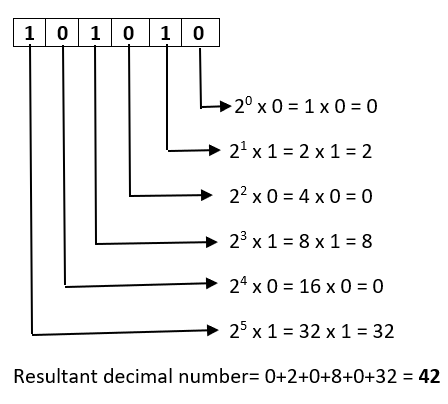
\includegraphics[scale=.5]{101010 binary.png}
\hfill \break

\subsection{Binary to Hexadecimal}
\textbf{Hexidecimal:} also known as hex, is the third commonly used number system. It has 16 units - 0-9 and the letters A, B, C, D, E and F.
\hfill \break

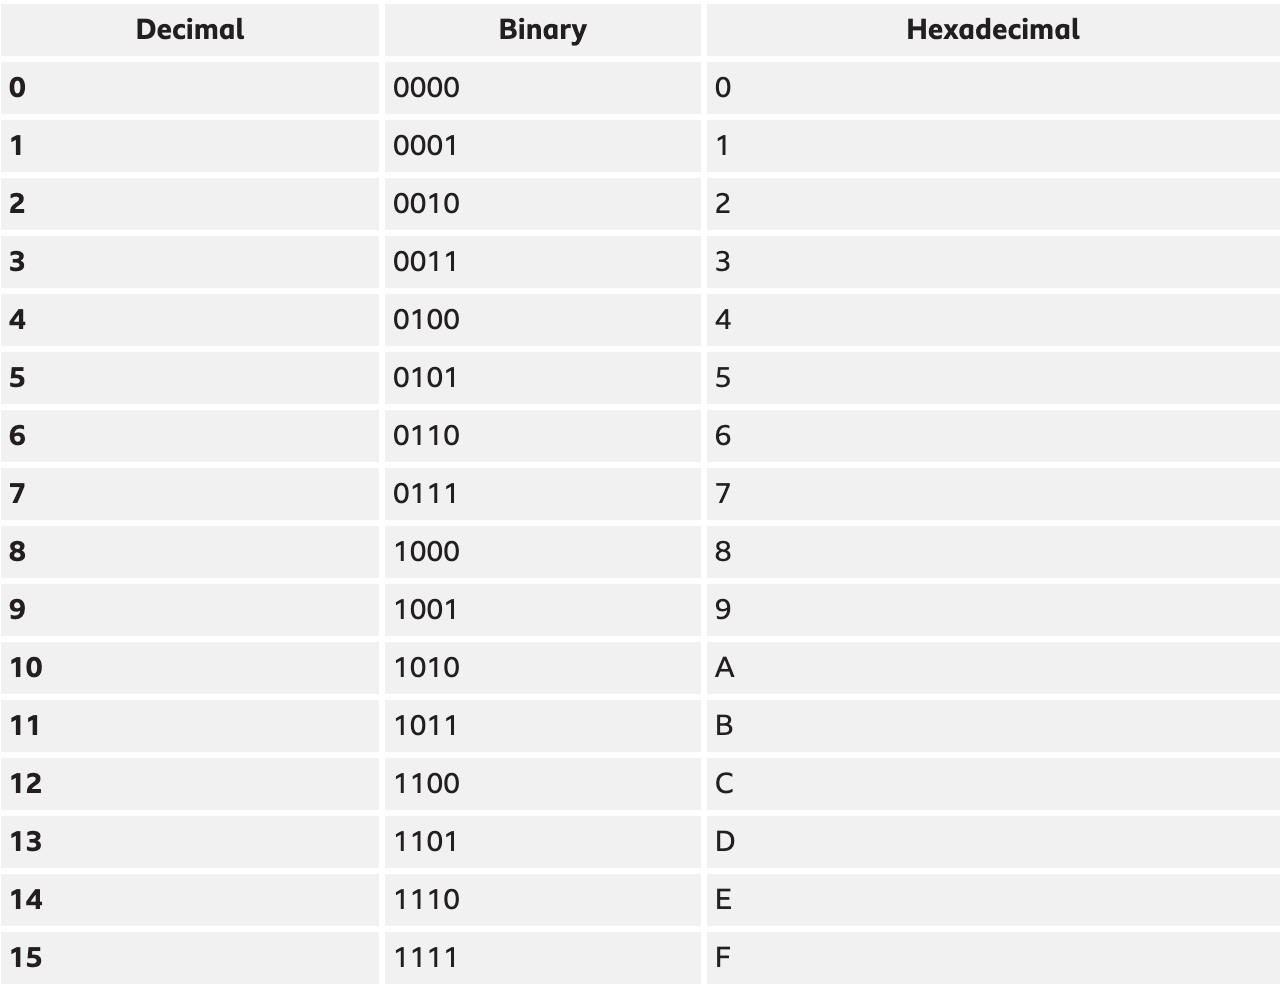
\includegraphics[scale=.5]{DBH Table.png}

\begin{enumerate}
    \item Start at the rightmost digit and break the binary number up into groups of four digits. These are known as nibbles. If there are less than four digits, use just that number of digits for that group.
    \item Next, convert each group of four digits into decimal. 
    \item Convert each decimal value into its hex equivalent. 
    \item Put the hex digits together.
\end{enumerate}

\textbf{Example:}

1101 to hex

1101 = decimal 13

13 = hex D

\vspace{5mm}
\section{Converting from Decimal}
\vspace{5mm}
\subsection{Decimal to Binary}
\textbf{Divide by 2 method}
\hfill \break
An easy method of converting decimal to binary number equivalents is to write down the decimal number and to continually divide-by-2 (two) to give a result and a remainder of either a “1” or a “0” until the final result equals zero.

\hfill \break

So for example. Convert the decimal number 29410 into its binary number equivalent.
\hfill \break
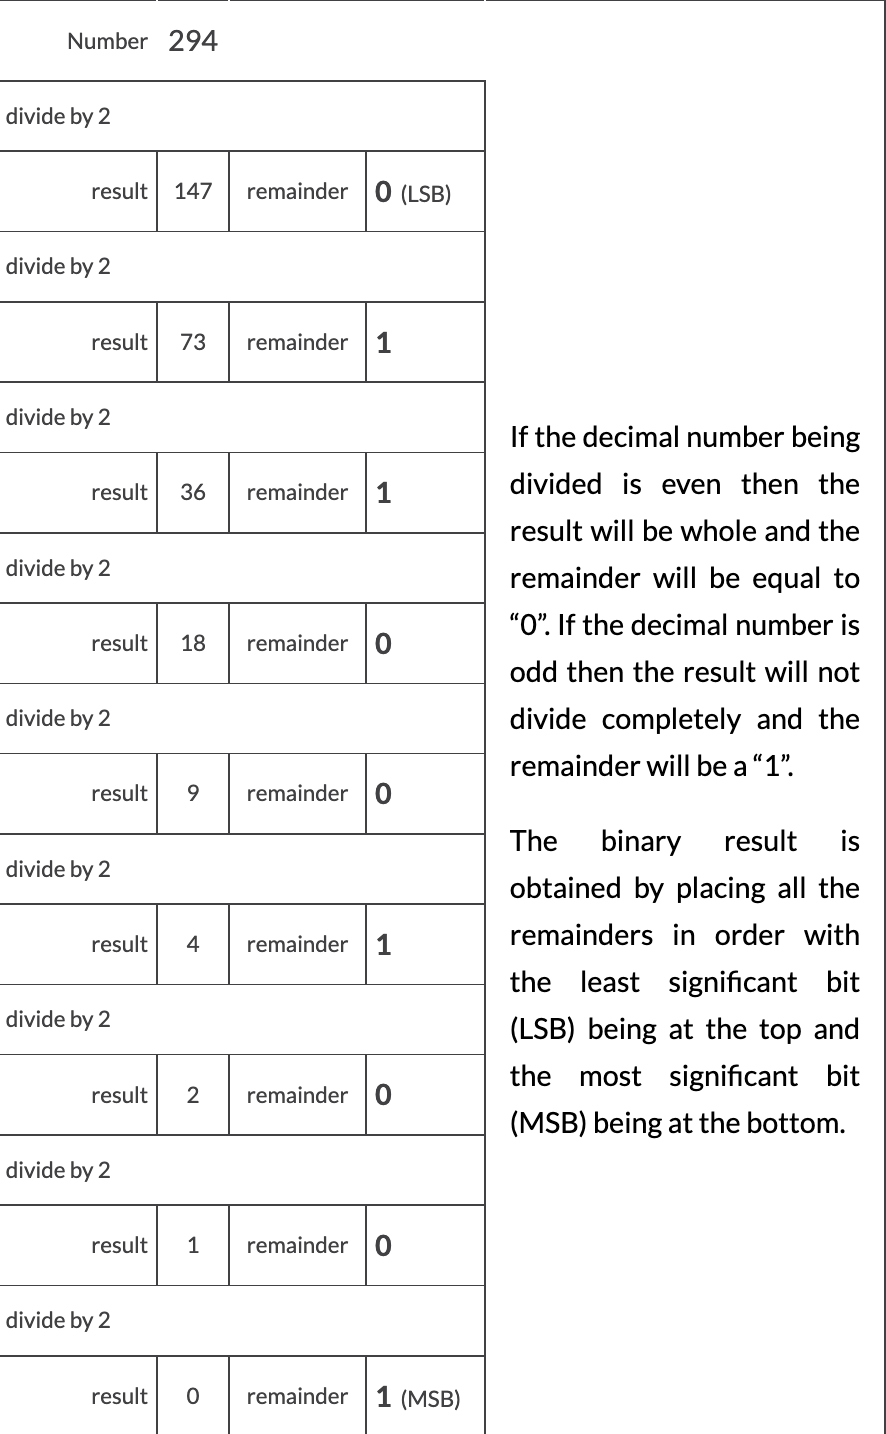
\includegraphics[scale=.5]{294.png}
\hfill \break

\subsection{Decimal to Hexadecimal}
\begin{enumerate}
    \item If the decimal number is bigger than 16, divide it by 16. Take the hexadecimal equivalent of this result - this represents the first digit. Take the hexadecimal equivalent of the remainder - this represents the second digit.
    \item If the decimal number is smaller than 16, take the hexadecimal equivalent of the decimal number.
\end{enumerate}

\hfill \break
\textbf{Example} - convert decimal 22 to hexadecimal
\hfill \break
16 goes into 22 once with 6 left over, so 22 ÷ 16 = 1 remainder 6
\hfill \break
1 = hex 1
\hfill \break
6 = hex 6
\hfill \break
\textbf{Result} - 16
\hfill \break
\textbf{Example} - convert 138 to hexadecimal
\hfill \break
138 ÷ 16 = 8 remainder 10
\hfill \break
8 = hex 8
\hfill \break
10 = hex A
\hfill \break
\textbf{Result} - 8A
\hfill \break

\subsection{Decimal to Octal}

To \textbf{convert decimal to octal}, we have to learn about both the number systems first. A number with base 8 is the octal number and a number with base 10 is the decimal number. Here we will convert a decimal number to an equivalent octal number. It is the same as converting any decimal number to binary or decimal to hexadecimal.

\hfill \break
In decimal to binary, we divide the number by 2, in decimal to hexadecimal we divide the number by 16. In case of decimal to octal, we divide the number by 8 and write the remainders in the reverse order to get the equivalent octal number.

\hfill \break
\textbf{Decimal Number:} All the numbers to the base ten are called decimal numbers. These are the commonly used numbers, which are 0-9. It has both integer part and the decimal part. It is separated by a decimal point (.). Numbers on the left of the decimal are integers and numbers on the right of the decimal is the decimal part. Example: (236.89)10, (54.2)10, etc.

\hfill \break
\textbf{Octal number:} These are the numbers with base 8. If x is a number then the octal number is denoted as x8. It contains digits from 0 to 7. Example: (212)8, (121)8, etc.

\vspace{8mm}
\hfill \break
Follow the steps given below to learn the decimal to octal conversion:

\begin{enumerate}
    \item Write the given decimal number
    \item If the given decimal number is less than 8 the octal number is the same.
    \item If the decimal number is greater than 7 then divide the number by 8.
    \item Note the remainder, we get after division
    \item Repeat step 3 and 4 with the quotient till it is less than 8
    \item Now, write the remainders in reverse order (bottom to top)
    \item The resultant is the equivalent octal number to the given decimal number.
\end{enumerate}

\hfill \break
\textbf{For example:} Convert 1792 into an octal number.

\hfill \break
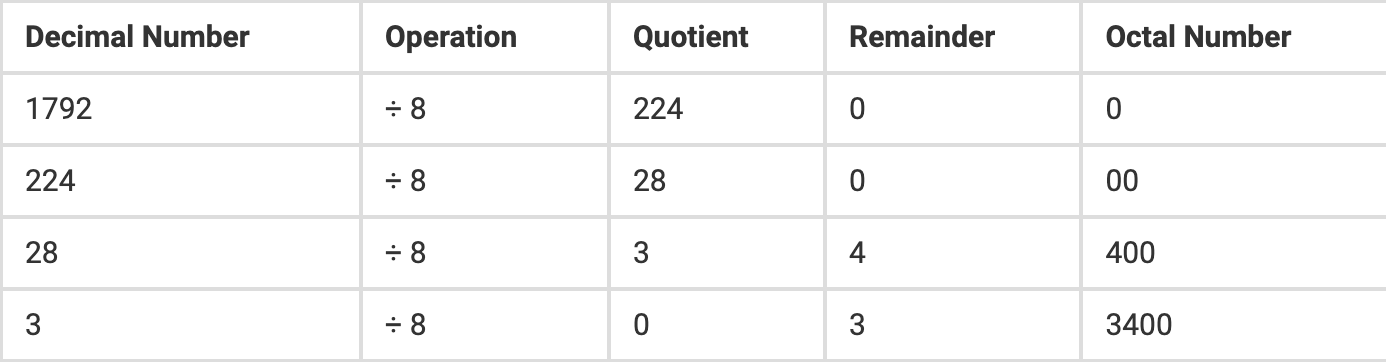
\includegraphics[scale=.5]{1792.png}

\hfill \break
\section{Converting from Hexadecimal}
\vspace{5mm}
\subsection{Hexadecimal to Binary}
\begin{enumerate}
    \item Split the hex number into individual values.
    \item Convert each hex value into its decimal equivalent.
    \item Next, convert each decimal digit into binary, making sure to write four digits for each value.
    \item Combine all four digits to make one binary number.
\end{enumerate}

\hfill \break
\textbf{Example} - hex 28 to binary
\hfill \break
2 = decimal 2 8 = decimal 8
\hfill \break
2 = binary 0010 8 = binary 1000
\hfill \break
\textbf{Result} - 00101000
\hfill \break
\textbf{Example} - hex FC to binary
\hfill \break
F = decimal 15 C = decimal 12
\hfill \break
15 = binary 1111 12 = binary 1100
\hfill \break
\textbf{Result} - 11111100

\hfill \break
\subsection{Hexadecimal to Decimal}

As we know, number systems can be converted from one base to another. Thus, we can convert hexadecimal numbers to decimal easily. This number system conversion can be done as explained in the example given below:

\hfill \break
\textbf{Example}:

\hfill \break
Convert 7CF (hex) to decimal.

\hfill \break
\textbf{Solution:}

\hfill \break
Given hexadecimal number is 7CF.

\hfill \break
In hexadecimal system,

\hfill \break
7 = 7

\hfill \break
C = 12

\hfill \break
F = 15

\hfill \break
To convert this into a decimal number system, multiply each digit with the powers of 16 starting from units place of the number.

\hfill \break
7CF = (7 × 162) + (12 × 161) + (15 × 160)

\hfill \break
= (7 × 256) + (12 × 16) + (15 × 1)

\hfill \break
= 1792 + 192 + 15

\hfill \break
= 1999

\hfill \break
From this, the rule can be defined for the conversion from hex numbers to decimal numbers.

\hfill \break
Suppose below is the hex number with n digits:

\hfill \break
dn-1 … d3 d2 d1 d0

\hfill \break
Multiply each digit of the hex number with its corresponding powers of 16 and add them such as:

\hfill \break
dn-1 × 16n-1 + … + d3 × 163 + d2 × 162 + d1 × 161 + d0 × 160

\hfill \break
Thus, the resultant number will be taken as base 10 or decimal number system.

\hfill \break
\textbf{Example 1:}
\hfill \break
Convert (1DA6)$_1_6$ to decimal.

\hfill \break
\textbf{Solution:}
\hfill \break
(1DA6)16

\hfill \break
Here,
\hfill \break
1 = 1
\hfill \break
D = 13
\hfill \break
A = 10
\hfill \break
6 = 6

\hfill \break
Thus,
\hfill \break
(1DA6)$_1_6$ = (1 × 163) + (13 × 162) + (10 × 161) + (6 × 160)
\hfill \break
= (1 × 4096) + (13 × 256) + (10 × 16) + (6 × 1)
\hfill \break
= 4096 + 3328 + 160 + 6
\hfill \break
= 7590

\hfill \break
Therefore, (1DA6)$_1_6$ = (7590)$_1_0$

\hfill \break
\textbf{Example} 2:
\hfill \break
Convert (E8B)$_1_6$ to decimal system.

\hfill \break
\textbf{Solution}:
\hfill \break
(E8B)$_1_6$

\hfill \break
Here,
\hfill \break
E = 14
\hfill \break
8 = 8
\hfill \break
B = 11

\hfill \break
Thus,
\hfill \break
(E8B)$_1_6$ = (14 × 162) + (8 × 161) + (11 × 160)
\hfill \break
= (14 × 256) + (8 × 16) + (11 × 1)
\hfill \break
= 3584 + 128 + 11
\hfill \break
= 3723

\hfill \break
Therefore, (E8B)$_1_6$ = (3723)$_1_0$
\hfill \break

\section{Other}
To \textbf{convert decimal to octal}, we have to learn about both the number systems first. A number with base 8 is the octal number and a number with base 10 is the decimal number. Here we will convert a decimal number to an equivalent octal number. It is the same as converting any decimal number to binary or decimal to hexadecimal.


\hfill \break
In decimal to binary, we divide the number by 2, in decimal to hexadecimal we divide the number by 16. In case of decimal to octal, we divide the number by 8 and write the remainders in the reverse order to get the equivalent octal number. ts-dudu,bs-dduu,tl-of3n1,bl-of1n2of1

\hfill \break
\textbf{Decimal Number:} All the numbers to the base ten are called decimal numbers. These are the commonly used numbers, which are 0-9. It has both integer part and the decimal part. It is separated by a decimal point (.). Numbers on the left of the decimal are integers and numbers on the right of the decimal is the decimal part. Example: (236.89)10, (54.2)10, etc

\hfill \break
\textbf{Octal number:} These are the numbers with base 8. If x is a number then the octal number is denoted as x8. It contains digits from 0 to 7. Example: (212)8, (121)8, etc.xor,and

\end{document}
